%% Copyright: National ICT Australia, 2005
%% Author   : Alexander Smola
%% License  : This file is licensed under the GNU Public License. See
%%            www.gnu.org for details on the license.
%%
%% This is a sample poster for the NICTA roadshow posters. Use it as
%% follows:
%%
%% \documentclass[landscape, a0]{nictaposter}
%% \columnfrac{0.31} %for three columns
%% \title{Title of the poster}
%% \staff{Authors} % or \staff{Staff List}
%% \program{Name of the NICTA Program}
%% \authors{First Name $|$ Second Name $|$ Third Name $|$ Fourth Name ... }
%% \content{This is where the content goes. It's a big minipage}
%%
%% add columns with
%%
%% \begin{pcolumn}
%% \section{Section level heading}
%% \subsection{Subsection level heading}
%%
%% whatever you want to write
%% \end{pcolumn}
%%
%% \begin{document}
%% \makeposter
%% \end{document}
%%
%% compile with 'pdflatex poster'

\documentclass[landscape, a0]{tumposter}
\usepackage{mdwlist,subfigure}
\usepackage{amsmath}
\usepackage{amssymb}
\usepackage{theorem}
\usepackage{graphicx}
\usepackage{natbib}
\usepackage{color}
%\usepackage{bbold}
\usepackage{hhline,url}
\usepackage{booktabs}
\usepackage[ruled,vlined]{algorithm2e}      
%\usepackage{epic,eepic}
%\usepackage{pstricks,pst-grad}
\graphicspath{{./}{./img/}}
\definecolor{MyLightGray}{rgb}{0.8,0.8,0.8}

\renewcommand{\bibsection}{}
\newcommand{\hess}[2]{\mathsf{H}_{#1}{(#2)}}

%------------------------------------------------------------
% number of columns in the poster:
%------------------------------------------------------------

\columnfrac{0.32}% three columns, each has width 0.3 times the textwidth

%%%%%%%%%%%%%%% local definitions %%%%%%%%%%%%%%%%%%%%%%%%%
\newcommand{\Fcal}{\mathcal{F}}
\newcommand{\Ncal}{\mathcal{N}}
\newcommand{\Xcal}{\mathcal{X}}
\newcommand{\Ycal}{\mathcal{Y}}
\newcommand{\Tcal}{\mathcal{T}}
\newcommand{\mymatrix}[2]{\left[\begin{array}{#1} #2 \end{array}\right]}
\newcommand{\NN}{\mathbb{N}}
\newcommand{\RR}{\mathbb{R}}
\newcommand{\tr}{\mathop{\mathrm{tr}\,}}
\newcommand{\one}{\mathbf{1}}
\newcommand{\tL}{\tilde{L}}

\newcommand{\ibkt}{\langle\alpha,e_{i}\rangle}
\newcommand{\bla}{\bigl\langle}
\newcommand{\bra}{\bigr\rangle}
\newcommand{\ov}{\overline}
\newcommand{\obkt}{\langle\alpha,e_{1}\rangle}
\newcommand{\abkt}{\langle\alpha,e_{j}\rangle}
\newcommand{\hlf}{\textstyle{\frac{1}{2}}}
\newcommand{\thrd}{\textstyle{\frac{1}{3}}}
\newcommand{\fth}{\textstyle{\frac{1}{5}}}
\newcommand{\sixth}{\textstyle{\frac{1}{6}}}
\newcommand{\norm}[1]{\lVert#1\rVert}
\newcommand{\mbs}{\boldsymbol}
\newcommand{\inv}{\operatorname{inv}}

\renewcommand{\top}{\mathsf{T}}		% matrix transpose
\newcommand{\cop}[1]{\overline{#1}}	% complex conjugate
\newcommand{\hop}{\mathsf{H}}		% Hermitian transpose
\newcommand{\dop}{\mathsf{\dag}}		% Generalized transpose

\DeclareMathSymbol{\C}{\mathbin}{AMSb}{"43}

%\theoremstyle{remark}
\theoremheaderfont{\scshape}
\newtheorem{lemma}{Lemma}
\newtheorem{theorem}{Theorem}
\newtheorem{define}{Definition}
%\newtheorem{Rem}{Remark}
\newtheorem{Cor}{Corollary}
\newtheorem{Ass}{Assumption}
\newtheorem{Prop}{Proposition}
\newtheorem{algorithm1}{Algorithm}%[section]
{\theorembodyfont{\rmfamily}
\newtheorem{Rem}{Remark}}
\newtheorem{Obs}{Fact}
\newenvironment{proof}{\noindent{\sc
Proof (Sketch).}\,\,}{\hfill\linebreak[0]\hspace*{\fill}}
%------------------------------------------------------------
% Now we start our poster:
%------------------------------------------------------------

%%%%%%%%% define headers %%%%%%%%%%%%
\title{\Huge Reinforcement Learning of Motor Skills with Policy Gradients}

%\subtitle{Performance by Optimisation}
\staff{\{amber.zhang, \}@tum.de } 
\program{Ruiming Zhang, }

%%%%%%%%% here goes the content %%%%%%%%%%%%%
\content{
\begin{pcolumn}

% this creates a column, you have to care yourself
% that it doesn't get too long for the poster

\section{Problem Setting}
\vspace*{-20mm}
%
{\large
\begin{itemize}
	\item Task: Learning complex motor skills with an anthropomorphic robot arm using reinforcement learning.\vspace{-2mm}
%

	\item Typical characteristics:
	\begin{itemize}
		\item  high-dimensional and continuous space and action space
		\item has to be model-free
		\item high degrees of freedom cannot deal with parameterised policies
	\end{itemize}
\end{itemize}
}

\section{Problem statement in Mathematics}
\vspace*{-20mm}
%
{\large
\begin{itemize}
% 	\item Assume that we can model the system in a discrete manner. Let $u_k \in R^M$ denotes the current action, $x_k, x_{k+1} \in R^N$ the current and the next state, then we can use a probability distribution:

% \begin{equation}
% 	x_{k+1} = p(x_{k+1} |x_k, u_k)
% \end{equation}

% 	\item Actions are generated by a policy:

% \begin{equation}
% 	u_k = \pi_\theta (u_k | x_k)	
% \end{equation}

	\item The general goal is to optimize the policy parameters $\theta \in R^K$ so that the expect return 
\begin{equation}
	J(\theta) = \frac{1}{a_\Sigma} E \{\sum_{k=0}^H a_k r_k\}
\end{equation}
is maximized. $a_k$ denote the time-step dependent weighting factors.
% optimized where $a_k$ denote time-step dependent weighting factors and $r_k$ the reward the learning system received by each instant of time.
\end{itemize}
\vspace*{2mm}
}

\subsection{Policy Gradient Method}
\vspace*{-17mm}
%
{\large
\begin{itemize}
	\item The policy parameter $\theta$ is updated at each time step by:
\begin{equation}
	\theta_{m+1} = \theta_m + \alpha_m \nabla_\theta J(\theta)
\end{equation}
where $\alpha_m \in R^+$ denotes a learning rate.
 % and fulfill:
% \begin{equation}
% 	\sum_{m=0}^\infty  \alpha_m > 0  \ \ and \  \ \sum_{m=0}^\infty \alpha_m^2 = 0
% \end{equation}
		%
	\item The main problem is obtaining a good estimator of the gradient $\nabla_\theta J |_{\theta=\theta_m}$.
\end{itemize}
}

\subsection{Likelihood Ratio Method}
\vspace*{-17mm}
{\large
%
\begin{itemize}
	\item Use $\tau$ to represent a real generated trajectory, $\tau \sim p_\theta(\tau) = p(\tau | \theta)$ , with rewards $r(\tau) = \sum_{k=0}^H a_k r_k$. Then the expect return of a policy can be written as an expectation over all possible trajectories:

\begin{equation}
	J(\theta) = \int p_\theta(\tau) r(\tau) d\tau
\end{equation}

 	\item Subsequently, the gradient can be rewritted by:
\begin{equation}
	\nabla_\theta J(\theta) = \int \nabla_\theta p_\theta(\tau) r(\tau) d\tau \nonumber \\
	= \int p_\theta(\tau) \nabla_\theta log p_\theta (\tau) r(\tau) d(\tau) \nonumber \\
	= E \{ \nabla_\theta log p_\theta (\tau) r (\tau)\}
\end{equation}

	\item The derivative $\nabla_\theta log p_\theta (\tau)$ can be computed by:

\begin{equation}
	\nabla_\theta log p_\theta (\tau) = \sum_{k=0}^H \nabla_\theta log \pi_\theta (u_k | x_k)
\end{equation}
	\item A constant baseline can be inserted since it has no effect to the derivative. Usually $b$ is chosen with the goal to minimize the variance of the gradient estimator. and results in the final form of the gradient estimator:
% \begin{equation}
% 	\nabla_\theta J(\theta) = E\{\nabla_\theta log p_\theta(\tau) (r(\tau) - b)\}
% \end{equation}
\begin{equation}
	\nabla_\theta J(\theta) = \left<\bigg(\sum_{k=0}^H \nabla_\theta log \pi_\theta (u_k | x_k)\bigg)\bigg(\sum_{l=0}^Ha_l r_l - b\bigg)\right>
\end{equation}

\end{itemize}
\vspace*{2mm}
}


\end{pcolumn}
%
\hfill
%%%%%%%%%%%%%%%%%%%%%%%%%%%%%%%%%
\begin{pcolumn}

% \subsection{Motor Primitive Framework}
% \vspace*{-17mm}
% %
% {\large
% \begin{itemize}
% 	\item We use motor commands to well represent a trajectory, which forms the stochastic policy:

% \begin{equation}
% 	\pi(\ddot{\hat{q_d}} | q_d) = \frac{1}{\sqrt{2 \pi \sigma^2}} exp(-\frac{(\ddot{\hat{q_d}} - \ddot{q_d})^2}{2 \sigma^2})
% \end{equation}

% The $\ddot{\hat{q_d}}$ term denotes for a perturbed target output considering the exploration controlled only through $\sigma$.
% 		%
% \end{itemize}
% }

\section{Natural Actor-Critic Algorithm}
\vspace*{-20mm}
%
{\large
\begin{itemize}
	\item We first introduce second-order Taylor expansion to approximate the closeness of two distribution, i.e. the amount of change of the policy: \vspace{-2mm}
\begin{equation}
	d_{KL} (p_\theta(\tau) \ || \ p_{\theta+\Delta_\theta}(\tau)) \approx \frac{1}{2} \Delta \theta^T F_\theta \Delta \theta
\end{equation}
where
\begin{equation}
	F_\theta = \int p_\theta(\tau) \nabla log p_\theta(\tau) \nabla log p_\theta (\tau)^T d\tau = \big<\nabla log p_\theta(\tau) \nabla log p_\theta(\tau)^T\big>
\end{equation}
is known as the Fisher information matrix.

\end{itemize}
\vspace*{2mm}
}

\subsection{Natural Gradient}
\vspace*{-17mm}
%
{\large
\begin{itemize}
	\item Assume that the amount of change is fixed using step size $\varepsilon$. Then the optimization problem can be described as:
\begin{eqnarray}
	& \max \limits_{\Delta\theta} J(\theta + \Delta\theta) \approx J(\theta) + \Delta\theta^T \nabla_\theta J \\
	& s.t.\  \varepsilon = d_{KL}(p_\theta(\tau) \ ||\ p_{\theta+\Delta\theta} (\tau) \approx \frac{1}{2} \Delta \theta^T F_\theta \Delta \theta)   \nonumber
\end{eqnarray}

and has the solution:
\begin{equation}
	\Delta \theta = \alpha_n F_\theta^{-1}\nabla_\theta J
\end{equation}
with $\alpha_n = [\varepsilon(\nabla J(\theta)^TF_\theta^{-1}\nabla J(\theta))^{-1}]^{\frac{1}{2}}$. 
	\item The item $\widetilde \nabla_\theta J(\theta) = \Delta \theta / \alpha_n$ is called the natural gradient and we will use it to replace the original gradient $\nabla_\theta J$ which represents the steepest ascend in order to obtain a faster convergence and stable update.

\end{itemize}
\vspace*{2mm}
}

\subsection{Compatible Function Approximation}
\vspace*{-17mm}
%
{\large
\begin{itemize}
	\item Use a compatible function approximation parameterized by $\omega$ to repalce the critic term:
\begin{equation}
	(\nabla_\theta log \pi(u | x))^T \omega = Q^\pi(x, u) - b^\pi(x)
\end{equation}
	\item  Thus we derive an estimte of the policy gradient as:
\begin{equation}
	\nabla_\theta J(\theta) = \int_x d^\pi(x) \int_u \nabla_\theta \pi(u | x)\nabla_\theta log \pi(u|x)^T dudx\omega = \int_x d^\pi(x)\hat{G_\theta}(x)dx\omega = G_\theta \omega
\end{equation}
	\item The left-undecided Fisher information matrix in last section can be determined through sampling:
\begin{eqnarray}
	& F_\theta = -\left<\nabla_\theta^2 log p(\tau_{0:H})\right> = -\left<\sum_{k=0}^H \nabla_\theta^2 log \pi(u_H | x_H)\right>  \nonumber \\
	& = - \int_x d_H^\pi (x) \int_u \pi(u|x) \nabla_\theta^2 log pi(u|x)dudx = G_\theta
\end{eqnarray}
	\item Thus the natural gradient can be simply computed as $\widetilde \nabla_\theta J(\theta) = F_\theta^{-1}G_\theta \omega = \omega$. Therefore the resulting policy improvement step becomes $\theta_{i+1} = \theta_i + \alpha\omega$.
\end{itemize}
\vspace*{2mm}
}
\subsection{Episodic Natural Actor-Critic Algorithm}
\vspace*{-17mm}

\end{pcolumn}
%
\hfill
%%%%%%%%%%%%%%%
\begin{pcolumn}
%
%%%%%%%%%%%%%%%%%%%%%%%%%%%%%%%%%%%%%%%%%

\vspace*{-28mm}
%
{\large
\begin{itemize}
	\item The Bellman equation can be witten in terms of 	the advantage function and the state-value function:
\begin{equation}
	Q^\pi (x, u) = A^\pi(x, u) + V^\pi(x) = r(x,u) + \gamma \int_x p(x^{'}|x,u)V^\pi(x^{'})dx^{'}
\end{equation}
	\item Inserting $A^\pi(x,u)$ as the compatible value approximation term and $V^\pi(x)$ an appropriate basis function representation $\phi(x)^Tv$ we have:
\begin{equation}
	\nabla_\theta log \pi(u_t|x_t)^T\omega + \phi(x_t)^Tv = r(x_t, u_t) + \gamma\phi(x_{t+1}^T)v + \varepsilon(x_t, u_t, x_{t+1})
\end{equation}
	\item  For episodic tasks we can derive a simplified form:
\begin{equation}
	\sum_{t=0}^H a_t \nabla log \pi(u_t, x_t)^Tw + J_0 = \sum_{t=0}^H a_t r(x_t, u_t)
\end{equation}
	\item This means for non-stochastic tasks we can obtain a natural gradient after dim$\theta + 1$ roll-outs using least-squares regression:
\begin{equation}
	\left[
	\begin{matrix}
		\omega \\
		J_0
	\end{matrix}
	\right] = (\Psi^T \Psi)^{-1}\Psi^T R
\end{equation}
with
\begin{eqnarray}
	& \Psi_i = \left[\sum_{t=0}^{H}a_t \nabla log \pi (u_t, x_t)^T, 1 \right] \\
	& R_i = \sum_{t=0}^{H}a_t r(x_t, u_t)
\end{eqnarray}

	\item In order to take time-variance rewards significantly better into account, we use a time-variant average rewards $\overline r = [\overline r_1, \overline r_2, ..., \overline r_K$ and then we have to solve:  \vspace{-2mm}
\begin{equation}
\left[
	\begin{matrix}
		g_{eNACn} \\
		\overline r
	\end{matrix}
	\right] = 
\left[
	\begin{matrix}
		F_2 & \overline \Phi \\
		\overline \Phi^T & mI_H
	\end{matrix}
	\right]
\left[
	\begin{matrix}
		g \\
		\overline r
	\end{matrix}
	\right]
\end{equation}
and finally obtained:
\begin{equation}
	b = Q^{-1}(\overline r - \overline \Phi^T F_2^{-1}g)
\end{equation}
with $Q^{-1} = m^{-1}(I_n + \overline\Phi^T(mF_2-\overline\Phi\overline\Phi^T)^{-1}\overline\Phi)$ and $\Phi$ is the eligibility matrix. 
\end{itemize}
\vspace*{-2mm}
}

\section{Experiments \& Conclusion}
\begin{itemize}
	\item Task: Applying the Episodic Natural Actor-Critic to a Sarcos Master Arm to hit a baseball.
	\item Figure(a) shows the average of the reward. The robot fail to reproduce the behavior at first. Subsequently the accuracy of the hitting angle is improved to hit properly after 200-300 trials.
\end{itemize}
\begin{center}
	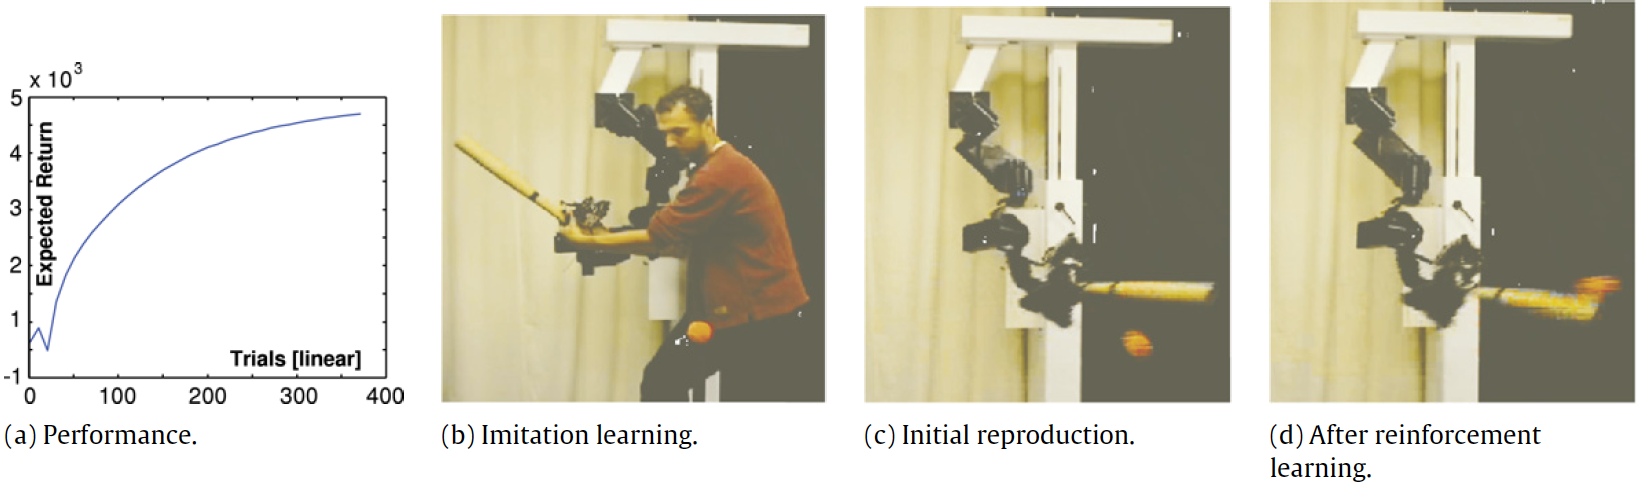
\includegraphics[width=0.9\textwidth]{img/performance1.png}
	\vspace*{-13mm}
\end{center}
\begin{itemize}
	\item Conclusion: The example of motor primitive learning for baseball underlines the efficiency of natural gradient methods for complex movement systems.
\end{itemize}


\end{pcolumn}
}

\notes{
%The CoTeSys Cluster of Excellence, M{\"u}nchen, Germany 
Research Group for Geometric Optimization and Machine Learning \\[3mm]
Technische Universit{\"a}t M{\"u}nchen, Germany}

\begin{document}
\makeposter
\end{document}
